\chapter{Systematic Uncertainties}
%\label{cha:SystematicUncertainties}
%\section{Systematic Error Estimations in \gones and \afone}
\label{sysErrsAll}


There is always a possibility that the final result(s) produced from any data analysis will be shifted from the true or ideally expected value(s) because the final result(s) are derived using the measured, modeled or estimated values of one or more other input parameters, whose values themselves usually have some systematic measurement or estimation uncertainties.

The systematic effects due to a particular variable are studied by making a small change in the variable while holding the others constant, and measuring by how much the end result(s) changed.

In this analysis, ten sources of systematic uncertainties are studied as listed below: %(labeled 0-12), they are given in table~\ref{tab:sysErrorSources} along with the number of variations and description for each source.
%Contributions from these 10 individual components are estimated and then a total contribution is estimated by first combining the corresponding individual compenents from the two beam energy (1.3 & 2.0 GeVs) data sets and finally combining them all by calculating the RMS of the ten combined contributions. The ten contributions are as follows:  (kp: 9/26/16 removed to minimize redundancy)

\begin{enumerate}
\label{TenSyUncertainties}          
\item Possible Uncertainty in the overall scaling factor
\item Effect due to the contaminations from polarized H in the target and from misidentified \pim in the scattered electrons sample.
%%\item Possible uncertainty in the beam energy measurement       
%%SEK: 9/30/16: I know we ``only'' vary the beam energy, but this is more generally meant to simulate kinematic mis-reconstruction (including imperfect momentum corrections, resolution, energy loss etc.). After all, by varying E we vary nu and Q2, which would also happen if we instead varied E' or theta. So maybe call it ``Potential deviations in the reconstructed kinematics''.
\item Potential deviations in the reconstructed kinematics
\item Possible uncertainty in the CC-inefficiency estimation
\item Effect due to the \epem pair symmetric contamination
%%\item Possible uncertainty in the estimation of radiation lengths (especially RADA) %\textcolor{red}{Why didn't we consider RADB? Lack of time or just minimal effect?}
%%SEK: 9/30/16: I wouldn't be too specific (``especially RADA''). What we really want to simulate is the uncertainty in radiative corrections from all other sources than the input models (which is done separately), with the dominant effects coming from the overall thickness in radiation lengths. 
\item Possible uncertainty in the estimation of radiation lengths
\item Model variation using preliminary version (v1) of $A_1$ model by Guler/Kuhn (2008-9) %(2008-9 (c)) % AsymChoice=12, SFchoic=11
%\textcolor{red}{How do I cite these models sources}
\item Model variation using old version of $A_2$ resonance model % AsymChoice=15, SFchoic=11
%\item Model variation of $F_2$ (and proportionally of $F_1$) %variation adding uncertainties to $F_2$ (and proportionally to $F_1$) % AsymChoice=11, SFchoic=12
%% SEK: 9/30/16: For 10, I believe we actually keep F2 constant and modify only F1, while for 9, we keep R constant and hence modify both F1 and F2.
\item Model variation of $F_2$ (and proportionally of $F_1$) while keeping R constant 
%\item Model variation of R ($F_2$ changed) %Model variation subtracting uncertainties from R ($F_2$ changed) % AsymChoice=11, SFchoic=13
\item Model variation of R or $F_1$ (with $F_2$ unchanged) %% See SEK comment above dated 9/30/16
\end{enumerate}
For the ease of description later on, these ten components will be referred to by the index "k" with its value indicating the position 
in the list. So, the uncertainty due to scaling factor will be identified with k=1 and so on.



\section{Evaluation of Experimental Systematics} %upon xz suggestion

\paragraph{Possible Uncertainty due to the overall scaling factor}
This uncertainty is due to the uncertainties in the overall scaling factor (SF), which is a convolution of various unmeasured constants such as \pbpt, packing fraction etc (see Sec. \ref{scaleerr}). This contribution is estimated by assuming that the uncertainties in SF is not more than 10\%. Thus considering the worst case scenario of 10\% uncertainty in SF, we estimate the corresponding uncertainty in \gones as follows:
\begin{equation}
\label{eqSysScl}
\Delta g_1^{SF}(W,Q^2) = g_1^{std}(W,Q^2) + \frac{\Delta n^{data}(W,Q^2) - 1.1 \cdot \Delta n^{std}(W,Q^2)}{1.1\cdot B(W,Q^2) } - g_1^{data}(W,Q^2)
\end{equation}
with ``std'' shorthand used for ``standard'' model or the corresponding simulation i.e. the ones provided by RCSLACPOL when
the asymmetry $A_1$ was not artificially increased to $A_1+0.1$. Here, $\Delta n^{data}$ and $\Delta n^{std}$ represent the 
polarized count differences for the experimental and simulated (without artificially changing $A_1$) data respectively.



\paragraph{Uncertainty from Polarized H in target and \pim contaminations}
\label{polBg}             

This contribution from polarized H in target and \pim contamination %\textcolor{red}{section reference} 
is evaluated as follows, 
\begin{equation}
\label{eqSysCont}
\Delta g_1^{cont}(W,Q^2) = g_1^{std}(W,Q^2) + \frac{\Delta n^{data}(W,Q^2)\cdot 1.025 - \Delta n^{std}(W,Q^2)}{B(W,Q^2) } - g_1^{data}(W,Q^2)
\end{equation}
where we assume that the contamination is not more than 2.5\%, which is consistent with what was found from our own study of the contamination. %\textcolor{red}{How did we come up with 1.025?}

\paragraph{Possible uncertainty in the beam energy measurement} 
\label{syErEb}  
%Eb4Ser=Eb+0.01 used in the DoEventSimData of wHisto*Steg*Data2.C (histo h1nwEnWcs[bb])
This contribution is evaluated assuming the uncertainty in beam energy measurement is not more than 10 MeV, so either the experimental data or the standard-simulation data can be analyzed assuming the beam energy was different by 10 MeV. In this analysis, the simulated data was analyzed assuming that the beam energy was 10 MeV more than that used during the event generation or simulation which was the same as that used for analyzing the experimental data. For example, for the lower beam energy data set, 1339 MeV was used to analyze the experimental data as well as to simulate the corresponding data, but during the analysis of the simulated data, the energy value used was 1349 MeV. Here, the change in energy results in changes in both \qsqs and W.
\begin{equation}
\label{eqSysEb}
\Delta g_1^{Eb}(W,Q^2) = g_1^{std}(W,Q^2) + \frac{\Delta n^{data}(W,Q^2) - \Delta n^{std}_{Eb+}(W,Q^2)}{B(W,Q^2) } - g_1^{data}(W,Q^2)
\end{equation}
where $\Delta n^{std}_{Eb+}$ is now the simulated $\Delta n^{std}$ obtained by analyzing the data from the standard simulation as usual but with a beam energy that was 10 MeV more than the standard value.

\paragraph{Possible uncertainty in the CC-inefficiency estimation}
\label{syErCC}       

This contribution is estimated by assuming a maximum of 50\% uncertainty in the estimated inefficiency as follows: %\textcolor{red}{section reference}
The the 50\% error is justified because the uncertainty in inefficiency is no more than 50\% for $nphe>2.5$ (see Fig. \ref{figccInefFits}).
\begin{equation}
\label{eqSysCC}
\Delta g_1^{Eb}(W,Q^2) = g_1^{std}(W,Q^2) + \frac{\Delta n^{data}(W,Q^2) - \Delta n^{std}_{0.5CCi}(W,Q^2)}{B(W,Q^2) } - g_1^{data}(W,Q^2)
\end{equation}
where $\Delta n^{std}_{0.5CCi}$ is now the simulated $\Delta n^{std}$ obtained after applying 50\% more inefficiency instead of the actually estimated value.

\paragraph{Possible uncertainty due to \epem pair symmetric contamination}
\label{syErEpEm}
The contribution due to \epem pair symmetric contamination is calculated as follows:
\begin{equation}
\label{eqSysPS}
\Delta g_1^{Eb}(W,Q^2) = g_1^{std} + \frac{\Delta n^{data}\cdot\frac{1}{1+f(e^+e^-)} - \Delta n^{std}}{B(W,Q^2) } - g_1^{data}(W,Q^2)
\end{equation}
where f(\epem) is the fraction of electrons in a given bin that come from pair-symmetric \epem produced as estimated with EG1b fit by N. Guler \cite{nGuler_th} (used the closest available energies).


\paragraph{Radiative correction uncertainty}
\label{sysRC}    
Here, we need to change the parameter that most influences radiative corrections, the number of radiation lengths before (RADB) and after (RADA) the scattering. By increasing both numbers by 10\%, % 5\%, 
we should have a safe upper limit on practically all uncertainties coming from the radiative procedure itself. But, to simplify the situation, we increased the RADA parameter in RCSLACPOL by 20\% and repeated the full-statistic simulation. %Correlate corresponding change in $\delta \sigma^{rad}$ from the RCSLACPOL output with the corresponding inferred change in $g_1$ for each bin.
As a result the simulated count difference in each kinematic bin changed from $\Delta n^{std}$ to a new value $\Delta n^{rad}$. This change can be converted to the corresponding inferred change in $g_1$ by using the same proportionality factors $B(W,Q^2)$ as used earlier in the \gones (or \afone) extraction/calculation. In other words, for a given kinematic bin this particular contribution to the systematic uncertainty is calculated as:
\begin{equation}
\label{eqSysRC}
\Delta g_1^{rad}(W,Q^2) =  g_1^{std} +  \frac{\Delta n^{data}(W,Q^2) - \Delta n^{rad}(W,Q^2)}{B(W,Q^2) }  - g_1^{data}(W,Q^2)
\end{equation}
where the proportionality factor $B(W,Q^2)$ for the bin is exactly the same as that used to calculate \gones earlier.



\section{Model uncertainties}
\label{sysMod}   
The remaining four components in the total systematic uncertainty (the last four in the list \ref{TenSyUncertainties}) account for the model uncertainty contributions. %For this purpose, we changed the values of two of the model parameters ``AsymChoice'' and ``SFchoice'' (each takes value of 11, in the standard case)\footnote{ List of options for the values of {\bf AsymChoice} and {\bf SFchoice}
For this purpose, we changed the values of two of the model parameters ``AsymChoice'' and ``SFchoice'' (each takes value of 11, in the standard case)

%For this purpose, we 
We repeated the full statistics simulation four more times by changing the values of two RCSLACPOL parameters ``AsymChoice'' and ``SFchoice'' (which controls the values of model asymmetries and the structure functions, with each taking a value of 11 in the standard case) one by one corresponding to the following four model variations: 
\begin{enumerate}
 \label{fourModelVariations} 
\item Variation-1: AsymChoice=12, SFchoic=11
\item Variation-2: AsymChoice=15, SFchoic=11
\item Variation-3: AsymChoice=11, SFchoic=12
\item Variation-4: AsymChoice=11, SFchoic=13
\end{enumerate}
 where, the different values of the two RCSLACPOL parameters correspond to the following model choices:
\begin{enumerate}
\item {\bf AsymChoice} values are used to determine specific $A_1$/$A_2$ models used in the RCSLACPOL program %\textcolor{red}{How do I cite these models sources}
\begin{enumerate}
\item 11: Standard Resonance Model 2008-9 Guler/Kuhn   %New Standard Resonance Model 2008-9 (c) Guler/Kuhn    
({\bf Used for standard simulation}) 
\item 12: Variation of $A_1$ model (earlier fit)  %Preliminary version (v1) of $A_1$ model - 2008-9 (c) Guler/Kuhn  
\item 15: Variation of $A_2$ resonance model: %Old version of $A_2$ resonance model: 
Vary the virtual photon asymmetry $A_2$ in the resonance region within its fit uncertainties. %This change affects both the radiative tail (to a small extent) and the Born cross section difference within a given bin and is {\bf un}correlated with any change in $g_1$. %SEK note
\end{enumerate}
\item {\bf SFchoice} values are used to determine specific $F_1$/$F_2$ models.
\begin{enumerate}
\item 11: %2009 version of $F^n_1$/$F^p_1$/$F^A_1$ by Peter Bosted/Eric Christie (c) 2009, HERMES {(\bf Used for standard simulation}) (A in $F^A_1$ denoting a generic nucleus of atomic number A).
2009 version of $F^n_1$/$F^p_1$/$F^d_1$ by Peter Bosted/Eric Christie 2009, HERMES {(\bf Used for standard simulation}) (with d in $F^d_1$ denoting a deuteron).
\item 12: Same version as 11, but with fit uncertainties added to $F_2$ (and proportionally $F_1$)
\item 13: Same version as 11, but with fit uncertainties subtracted from R ($F_2$ unchanged)
\end{enumerate}
\end{enumerate}
 

%============ Keep this commented block for future reference purpose
\begin{comment}
\begin{enumerate}
\item {\bf AsymChoice} values (used to determine specific A1/A2 models used in the RR)
\begin{enumerate}
\item 11: New Standard Resonance Model 2008-9 (c) Guler/Kuhn     ({\bf Used for standard simulation})
\item 12: Preliminary version v1 of A1 model - 2008-9 (c) Guler/Kuhn
\item 15: Old version of A2 resonance model: 
Vary the virtual photon asymmetry $A_2$ in the resonance region within its fit uncertainties. This change affects both the radiative tail (to a small extent) and the Born cross section difference within a given bin and is {\bf un}correlated with any change in $g_1$. %SEK note
\end{enumerate}
\item {\bf SFchoice} values
\begin{enumerate}
\item 11: 2009 version of F1n/F1p/F1A by Peter Bosted/Eric Christie (c) 2009, HERMES {(\bf Used for standard simulation})
\item 12: Same version as 11, but with uncertainties added to F2 (and proportionally F1)
\item 13: Same version as 11, but with uncertainties subtracted from R (F2 unchanged)
\end{enumerate}
\end{enumerate}
\end{comment} 
%============ Keep this commented block for future reference purpose


 %Both of these parameters use 11 for standard simulation and other values are used one by one (keeping other things the same) for different simulations in order to estimate the sytematic uncertainties from each as follows:
After the simulation data for the above four cases (see \ref{fourModelVariations}) were available, four more data tables (TM1,TM2,TM3 and TM4) were produced for the corresponding model values of \gone, \aone, \fones etc. Then, the contributions to the systematic uncertainty from each of these four cases of model variation were given as follows:
\begin{equation}
\label{eqSysMd}
\Delta g_1^{i}(W,Q^2) = g_1^{std}(W,Q^2) - g_1^{i}(W,Q^2) + \frac{\Delta n^{i}(W,Q^2) - \Delta n^{std}(W,Q^2)}{B(W,Q^2) }
\end{equation}
with ``i'' indicating any of the four cases of model variation, $g_1^i$ being the model prediction for the $i^{th}$ case as obtained from the corresponding data table ``TMi'' and the proportionality factor $B(W,Q^2)$ again being exactly the same as used to calculate \gones as earlier.



\section{Combining uncertainties}
%see pdf-pg 179 in my thesis (where I talk about combining both data and uncertainties)
Contributions from the 10 individual components are estimated and then a total contribution is estimated by first combining the corresponding individual compenents for each of the two beam energies %energy (1.3 \& 2.0 GeVs) data sets 
and finally combining them all by calculating the RMS of the ten combined contributions.

\subsection{Combining uncertainties from the two beam energies}
In principle, each of the individual contributions to the systematic uncertainty can also be combined using the same equations as for combining \gones and \afones (see above). However, we must be careful to distinguish between correlated and uncorrelated uncertainties. 
If for a given $(W,Q^2)$ bin, %\gone or \afone comes 
data is available only from one beam energy, then combined uncertainty for the \kth component is simply the uncertainty from that beam energy. If there are measurements from both beam energies, we combine them with statistical weights as follows: 

\begin{enumerate}
\item The variations due to scale factor (k=1), beam energy (k=3) and CC-efficiency (k=4) are all un-correlated and, therefore, added in quadrature as follows:
\begin{eqnarray}
\label{eqSeUncorEb78Comb}
\delta g_1(\text{k=8,10,11, combined}) = \sqrt{ \left( \sum_i \frac{ (\delta g_1)^2(i)} {(\Delta g_1)^2(i)} \right)  / Sum2 }
\end{eqnarray}	
where, $\delta$ represents the \kth component of the systematic uncertainty, whereas, 'Sum2', 'i' and $\Delta$ have the same meanings as before, with 'Sum2' given by 
\begin{eqnarray}
\label{eqDataComb}
 Sum2 =  \sum_i \frac{1}{(\Delta g_1)^2(i)} 
\end{eqnarray}	
which provides the statistical weight, where the index 'i' represents two beam energy (1.3 and 2.0 GeV) data sets, %\text{with i=1.3 and 2.0 GeV}   \\  
and $\Delta g_1$ indicates the statistical uncertainty in \gone in the corresponding kinematic bin.

\item All other variations are correlated between the two beam energies and should be averaged linearly (WITH sign): 
\begin{eqnarray}
\label{eqSeUncorEb78Comb2}
\delta g_1(\text{other k, combined}) =  \left( \sum_i \frac{ (\delta g_1)(i)} {(\Delta g_1)^2(i)} \right)  / Sum2 
\end{eqnarray}	
\end{enumerate}



\subsection{Combining uncertainties from the ten sources}
Once each of the $k^{th}$ component of the systematic uncertainties are combined between the two beam energies, we then proceed to combine them all to get a grand total. This is done by simply adding the ten $E_b$-combined systematic uncertainties in quadrature and taking the square-root of the sum % \textcolor{red}{Reference to an example figure}
as follows:

\begin{eqnarray}
\label{eqErrCombAll}
 Total Systematic Uncertainty = \sqrt{ \sum^{10}_{k=1} (\Delta g_1)^2_k }
\end{eqnarray}










%\textcolor{red}{I could manage to enlarge and update some figures, but not all. I will work on them, most likely after 11/14.}
\begin{figure}[h] 
\centering
\subfigure[Breakdown of systematic errors]{
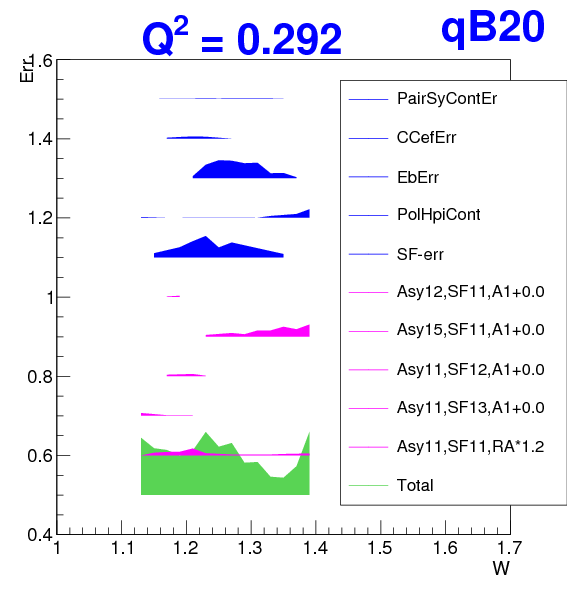
\includegraphics[width=0.49\textwidth]{figuresEG4/FigAnal/indvSystErrsEb7Wbins70NoG1N3pass2.png} 
\label{figSysErrs}
}
\subfigure[Extracted \gone in the corresponding bin]{
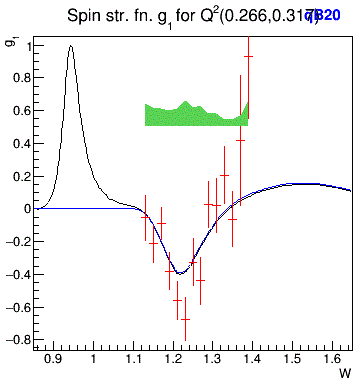
\includegraphics[scale=0.49]{figuresEG4/FigAnal/g1_stdAndExtracted_StdD79_nStdD80C71S181Eb7NoQe70WbinsCropped20thBin.png}
\label{figCorrespG1}
}



  %\leavevmode 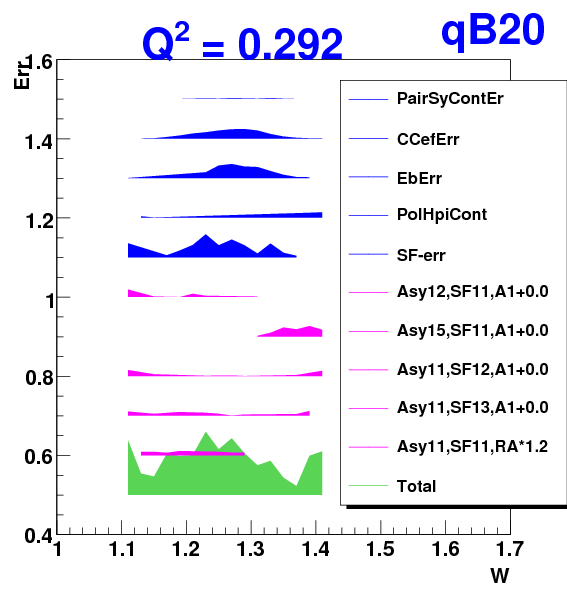
\includegraphics[width=0.9\textwidth]{figuresEG4/FigAnal/indvSystErrsEb7Wbins70NoG1N3.png} 
%\leavevmode 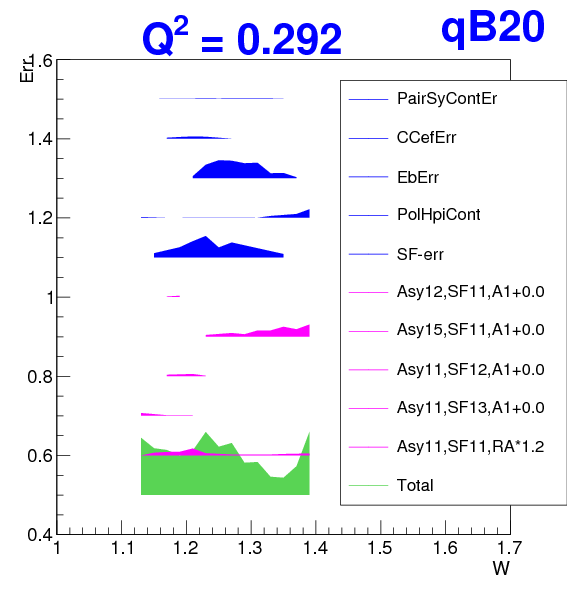
\includegraphics[width=0.9\textwidth]{figuresEG4/FigAnal/indvSystErrsEb7Wbins70NoG1N3pass2.png}
%xz: too many Sec. references in version 2 note (most always showed up as Sec 5), so I disabled most of them.
\caption[Breakdown of systematic uncertainties on \gones for 1.3 GeV]{On the left: various components of systematic uncertainty (see Sec. \ref{sysErrsAll} %and \ref{TenSyUncertainties})
  on \gones plotted against $W$ in a \qsqs bin (1.3 GeV data). The band width represents the size of the uncertainties. The vertical position of each band has no physical meaning (arbitrarily chosen for the convenience of display). The first five (blue) bands are the contributions due to \epem-contamination % (see Sec. \ref{syErEpEm})
  , CC-inefficiency %(see Sec. \ref{syErCC})
  , uncertainties in beam energy measurement %(see Sec. \ref{syErEb})
  , polarized background (H, \pim etc %- see Sec. \ref{polBg}
  ) and scaling factor uncertainties %(see Sec. \ref{scaleerr})
  respectively. The first (top) magenta band is the contribution due to the uncertainties in the radiative corrections %(see Sec. \ref{sysRC})
  , next four (magenta) are due to model uncertainties %(see Sec. \ref{sysMod})
  and the last (green) one is the total uncertainty after properly combining all components. For similar plots in other \qsqs bins see Figs. \ref{sysErEb7} and \ref{sysErEb7n}. On the right: extracted \gones vs W shown along with the total systematic uncertainty.} %{sysErrsAll}{TenSyErrors}  {scaleerr} {polBg} {syErEb}{syErCC} {syErEpEm}{sysRC}{sysMod}
  \label{sysErEb7q1}  
\end{figure}


\begin{figure}[h] 
\centering
  \leavevmode 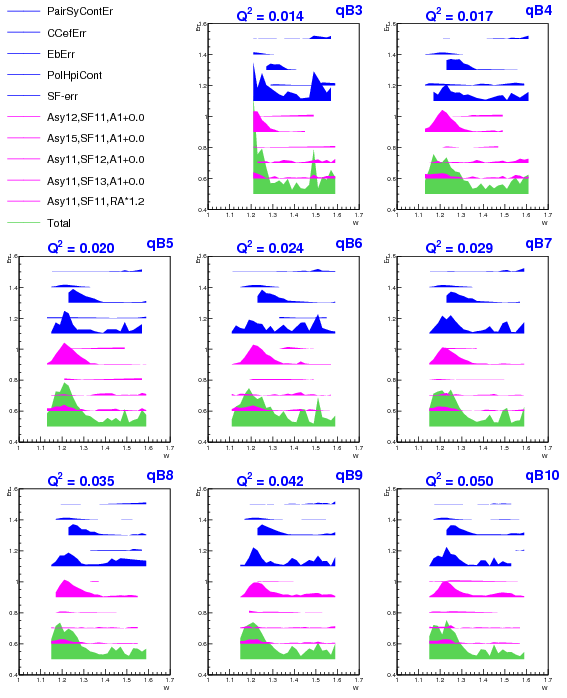
\includegraphics[width=0.9\textwidth]{figuresEG4/FigAnal/indvSystErrsEb7Wbins70NoG1Npass2.png} 
  \caption[Breakdown of systematic uncertainties on \gones for 1.3 GeV]{Plots like that shown in Fig. \ref{sysErEb7q1} showing various components of systematic uncertainty on \gones plotted against $W$ in different \qsqs bins for 1.3 GeV data.}
  \label{sysErEb7}  
\end{figure}

\begin{figure}[h] 
\centering
  \leavevmode 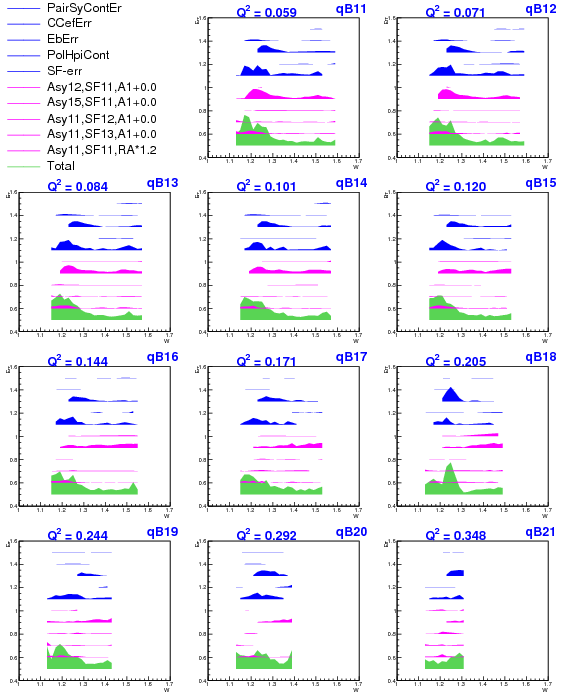
\includegraphics[width=1.0\textwidth]{figuresEG4/FigAnal/indvSystErrsEb7Wbins70NoG1N2pass2.png} 
  \caption[Systematic uncertainties in more bins (1.3 GeV)]{Systematic uncertainty components in remaining \qsqs bins (continuation of Fig. \ref{sysErEb7}.}
  \label{sysErEb7n}  
\end{figure}

Figs. (\ref{sysErEb7} and \ref{sysErEb7n}) show, for example, the different components of the systematic uncertainties along with the grand total on \gones (from 1.3 GeV data) evaluated in the manner just outlined. Likewise, Figs. (\ref{sysErEb8} and \ref{sysErEb8n}) show similar plots for the 2.0 GeV data.

\begin{figure}[h] 
\centering
  \leavevmode 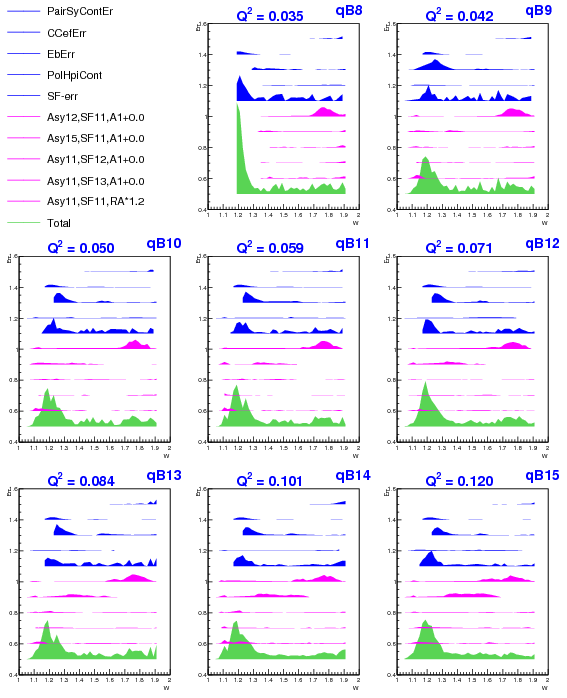
\includegraphics[width=0.9\textwidth]{figuresEG4/FigAnal/indvSystErrsEb8Wbins70NoG1Npass2.png} 
  \caption[Breakdown of systematic uncertainties on \gones for 2.0 GeV]{Plots similar to those shown in Fig. \ref{sysErEb7} but for 2.0 GeV, showing various components of systematic uncertainty on \gones plotted against $W$ in different \qsqs bins.}
  \label{sysErEb8}  
\end{figure}

\begin{figure}[h] 
\centering
  \leavevmode 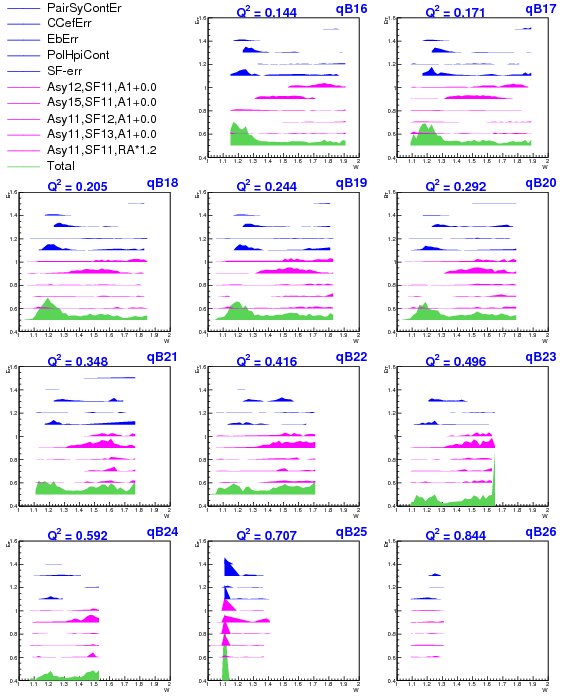
\includegraphics[width=1.0\textwidth]{figuresEG4/FigAnal/indvSystErrsEb8Wbins70NoG1N2pass2.png} 
  \caption[Systematic uncertainties in more bins (2.0 GeV)]{Systematic uncertainty components in remaining \qsqs bins (continuation of Fig. \ref{sysErEb8}.}
  \label{sysErEb8n}  
\end{figure}

These ten different components of systematic uncertainties on \gones and similarly on \afone thus calculated separately for both beam energies are later combined % in quadrature with proper statistical weighting to get the combined components as well as the grand total as shown 
as described below.


\subsection{Combining data from the two beam energies}
Once the data \gones and \afones and their corresponding uncertainties are evaluated from each beam energy data set, they are combined as follows \cite{pComKuhn} (to make the description simple, the procedure is described only for \gone, but, in the end, the exact same procedure is followed for \afones as well):

\begin{enumerate}
\item First a table is made, separately for each beam energy, of all $(Q^2,W)$ bins with calculated values of \gone, their statistical uncertainties and each of the ten components of the systematic uncertainties (making sure to keep the correct signs of the systematic changes).% in separate columns (one row is for one bin in $(Q^2,W)$. 
\item Then another table is made for the combined values of \gone, which are evaluated as follows:
\begin{enumerate}
\item If for a given $(W,Q^2)$ bin, \gones comes only from one beam energy, then all the entries from that energy go into the "combined" table
\item If \gones has measurements from both beam energies, we combine them with statistical weights as follows:
  
\begin{eqnarray}
\label{eqDataComb}
%Sum1 &=&  \sum_i \frac{g_1(i)}{(\Delta g_1)^2(i)}  \qquad         Sum2 =  \sum_i \frac{1}{(\Delta g_1)^2(i)} \\        
%g_1(combined) &=& Sum1 / Sum2                      \qquad         \sigma g_1(combined) = \sqrt{1/Sum2} 
Sum1 &=&  \sum_i \frac{g_1(i)}{(\Delta g_1)^2(i)}  \\
%Sum2 &=&  \sum_i \frac{1}{(\Delta g_1)^2(i)} \\    %xz asked to disabled it    
g_1(combined) &=& Sum1 / Sum2 \\
\sigma g_1(combined) &=& \sqrt{1/Sum2}
\end{eqnarray}	
where the index 'i' represents two beam energy (1.3 and 2.0 GeV) data sets, %\text{with i=1.3 and 2.0 GeV}   \\  
 $\Delta g_1$ indicates the statistical uncertainty in \gone and $Sum2$ is again given by Eq. \ref{eqDataComb} above..
\end{enumerate}
\item In principle, each of the individual contributions to the systematic uncertainty can also be combined using the same equations. However, we must be careful to distinguish between correlated and uncorrelated uncertainties. 
\begin{enumerate}
\item The variations due to scale factor (k=1), beam energy (k=3) and CC-efficiency (k=4) are all un-correlated and, therefore, added in quadrature as follows:
\begin{eqnarray}
\label{eqSeUncorEb78Comb}  %xz saw problem with k=8,10,11, and I don't know why I had these numbers.
%\delta g_1(\text{k=8,10,11, combined}) = \sqrt{ \left( \sum_i \frac{ (\delta g_1)^2(i)} {(\Delta g_1)^2(i)} \right)  / Sum2 } 
\delta g_1(\text{k=1,3,4, combined}) = \sqrt{ \left( \sum_i \frac{ (\delta g_1)^2(i)} {(\Delta g_1)^2(i)} \right)  / Sum2 }
\end{eqnarray}	
 where, $\delta$ represents the $k^{th}$ component of the systematic uncertainty, whereas, 'Sum2', 'i' and $\Delta$ have the same meanings as before.
\item while all other variations are correlated between the two beam energies and should be averaged with linear weighting (WITH sign): 
\begin{eqnarray}
\label{eqSeUncorEb78Comb2}
\delta g_1(\text{other k, combined}) =  \left( \sum_i \frac{ (\delta g_1)(i)} {(\Delta g_1)^2(i)} \right)  / Sum2 
\end{eqnarray}	
\end{enumerate}
%\textcolor{red}{Reference to an example figure}
\item Once each of the $k^{th}$ component of the systematic uncertainties are combined between the two beam energies, we then proceed to combine them all to get a grand total. This is done by simply adding the ten combined systematic uncertainties in quadrature and taking the square-root. % of the sum. % \textcolor{red}{Reference to an example figure}
\end{enumerate}






%Moved from Results section back to here 11/28/13 (I think that's what Dr. Kuhn suggested)
%\section{Systematic Uncertainties in the Extracted \gones, \afones}


Figures \ref{extG1SEcomb} and \ref{extA1F1SEcomb} show the breakdown of the total contribution to the systematic uncertainty from different sources. We can see that the dominant contribution comes from the uncertainties in the overall scale factor (the cyan band indicated with SF-err in the legend) which is used to normalize the simulated data to make them comparable with data. One of the big part of this uncertainty comes from those in $P_bP_t$ and target size measurements. Next big contributions seem to come from the model (in particular the model for the unmeasured $A_2$) and radiative corrections. Near the $\Delta$-resonance region, the effect of beam energy uncertainty also seems to be very pronounced. 
%Showing only systematic uncertainties (breakdonw of the 10 components for the beam-energy-combined data)
The breakdown of the different components (but combined between the two beam energies) of the total systematic uncertainties are also shown separately in the Figs. \ref{extG1SEcomb} and \ref{extA1F1SEcomb}.

\begin{figure}[h] %ht, htpb (p - float, b = bottom, h=? t = top)
\centering
  %\leavevmode 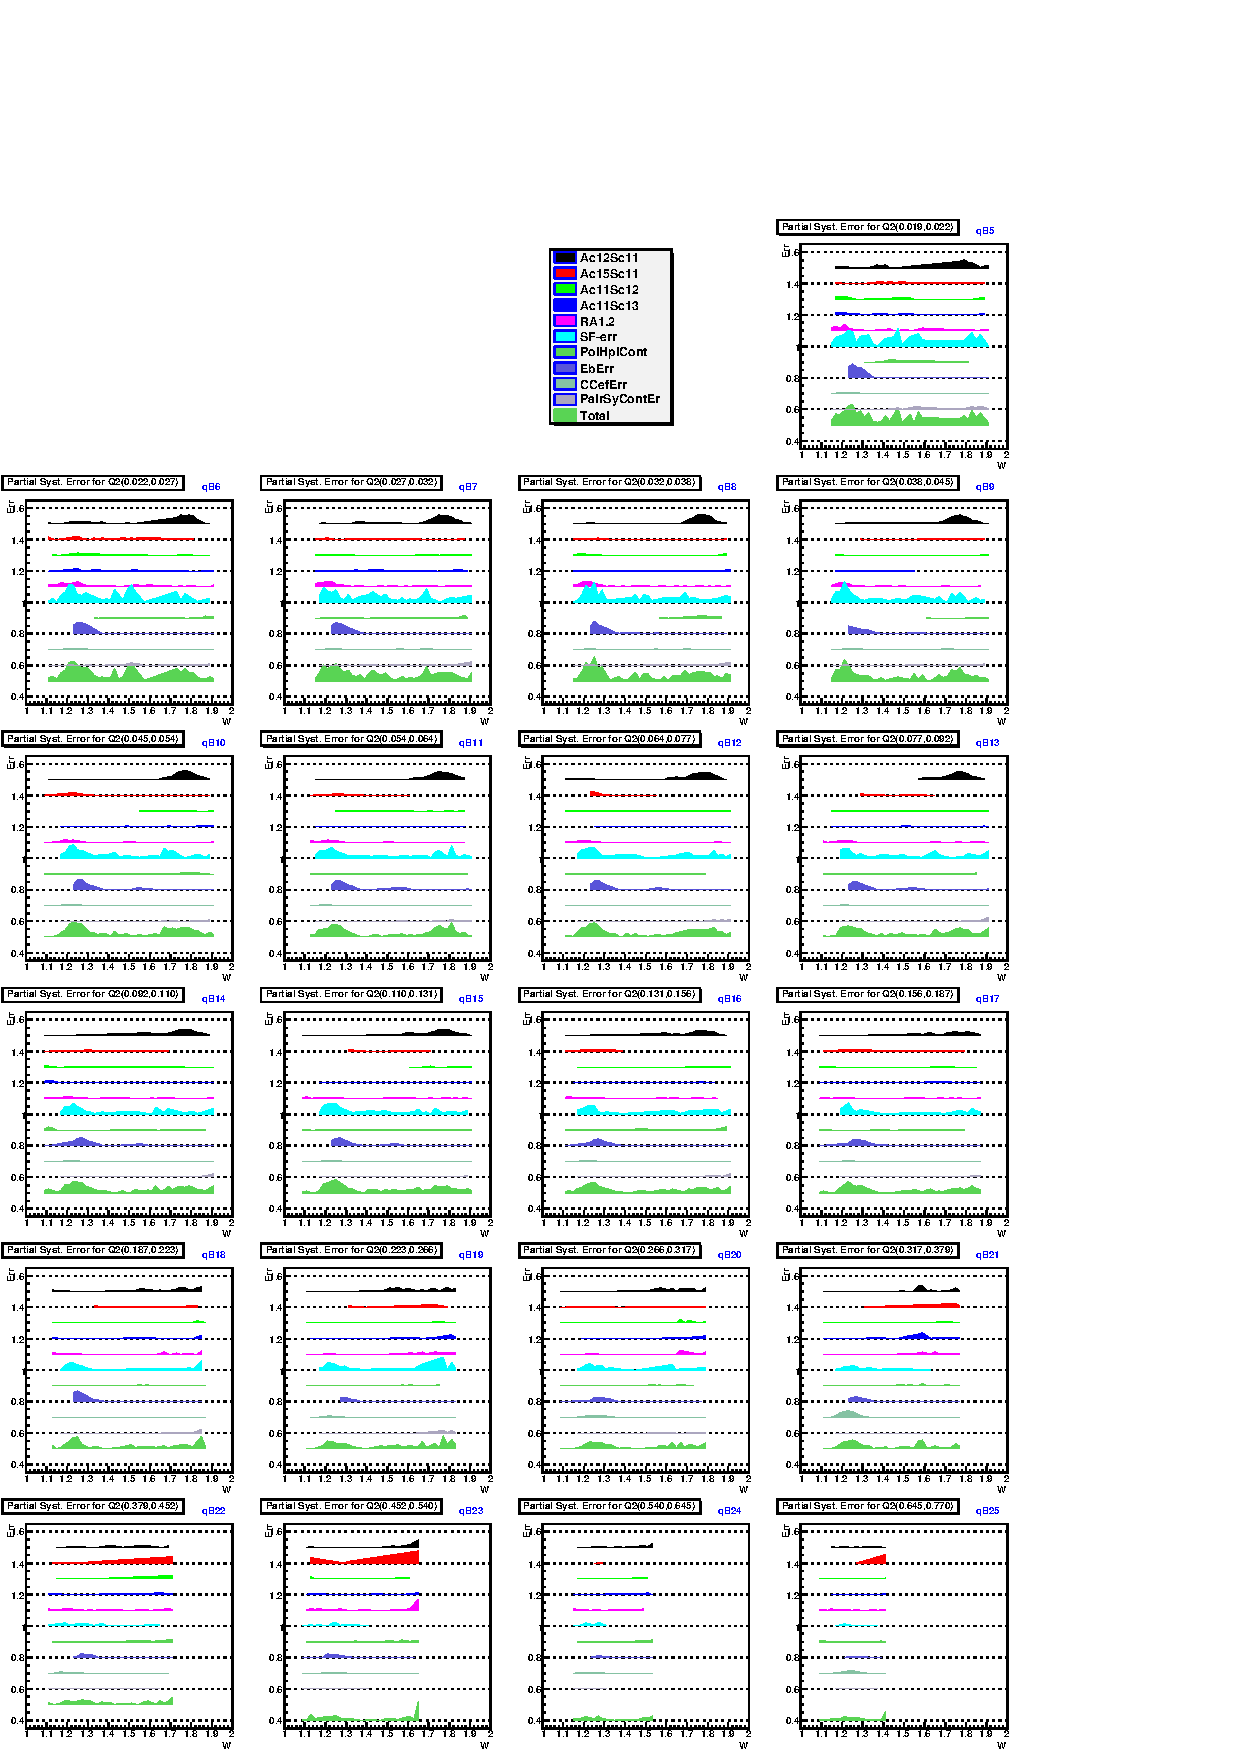
\includegraphics[width=0.95\textwidth]{figuresEG4/FigResults/indvSystErrsG1_Eb78Wbins70.png} 
  \leavevmode 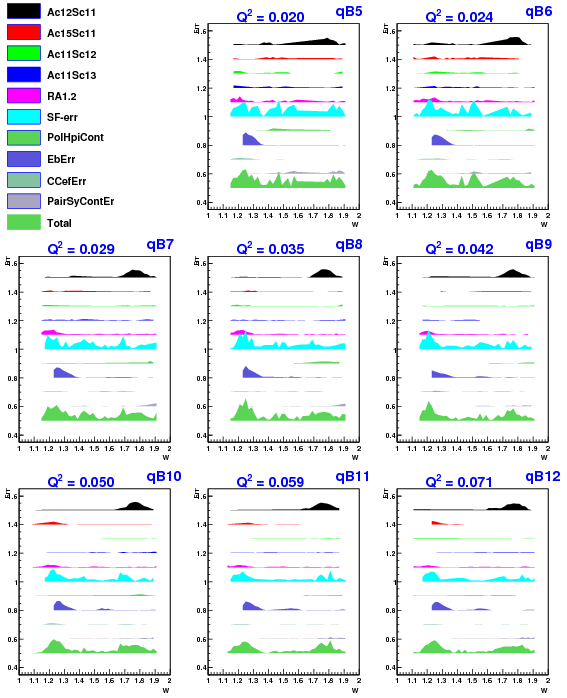
\includegraphics[width=0.95\textwidth]{figuresEG4/FigResults/indvSystErrsG1_Eb78Wbins70N.png} 
  \caption[Combined systematic uncertainties in $g_{1}$]{Breakdown of systematic uncertainties in $g_{1}$ (after combining data from the two energy data sets) in the first few \qsqs bins. See Fig. \ref{sysErEb7q1} for the description of the different systematic uncertainty components.}
  \label{extG1SEcomb} 
\end{figure}

\begin{figure}[h] %ht, htpb (p - float, b = bottom, h=? t = top)
\centering
  %\leavevmode 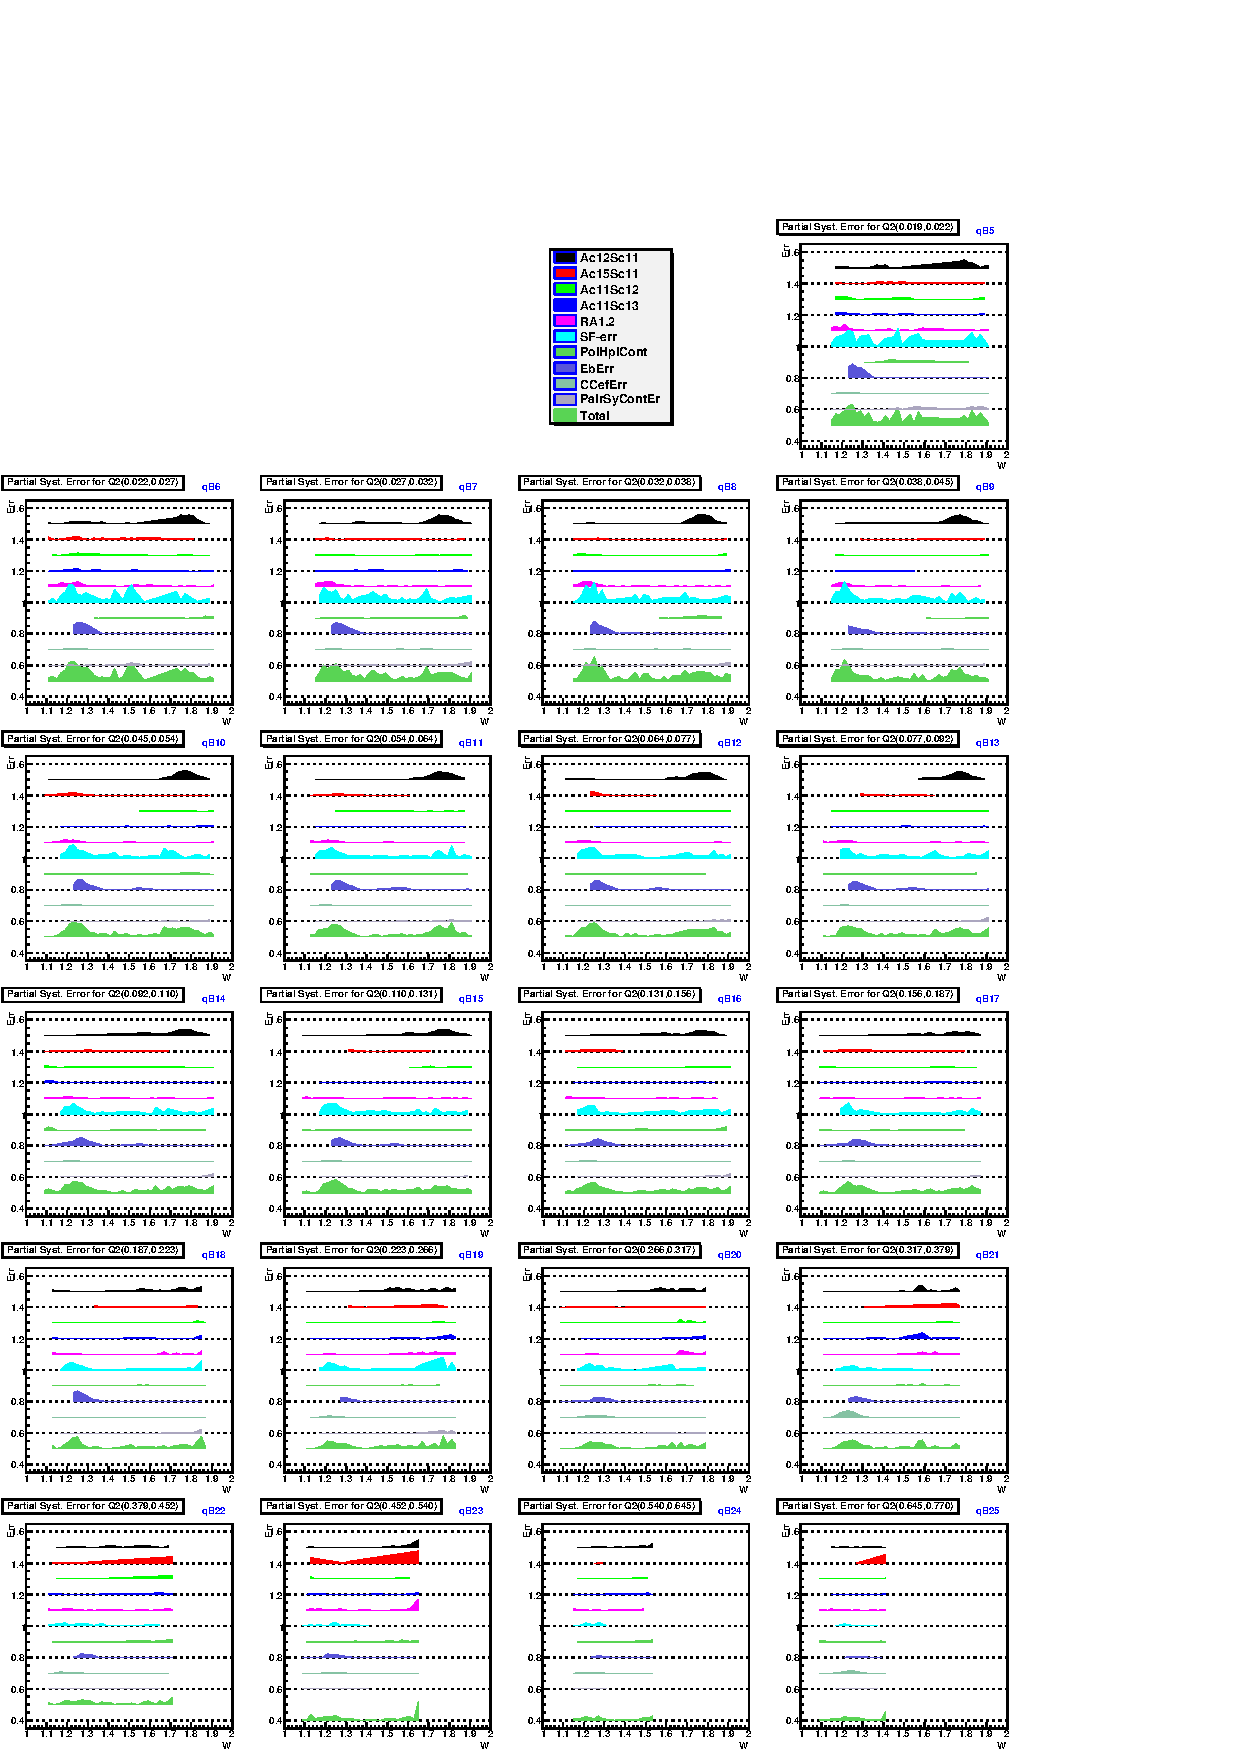
\includegraphics[width=0.95\textwidth]{figuresEG4/FigResults/indvSystErrsG1_Eb78Wbins70.png} 
  \leavevmode 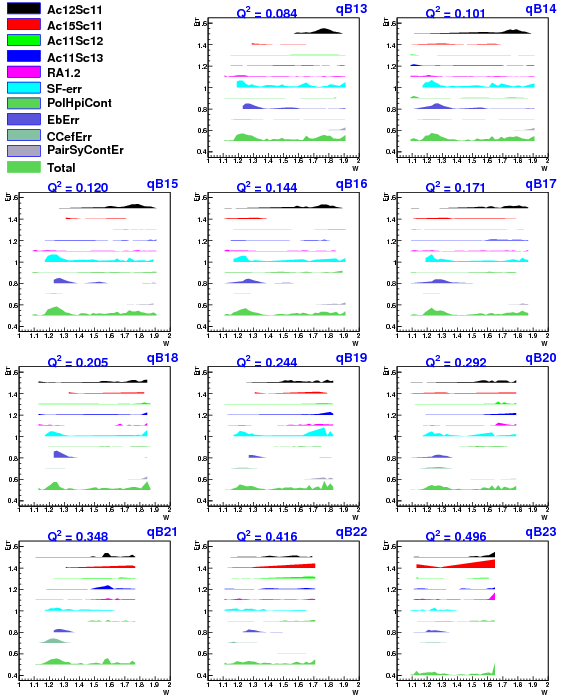
\includegraphics[width=0.95\textwidth]{figuresEG4/FigResults/indvSystErrsG1_Eb78Wbins70N2.png} 
  \caption[Combined systematic uncertainties in $g_{1}$]{Plots as in Fig. \ref{extG1SEcomb}  but in the remaining higher \qsqs bins.}
  \label{extG1SEcomb2} 
\end{figure}



\begin{figure}[h] %ht, htpb (p - float, b = bottom, h=? t = top)
\centering
  %\leavevmode 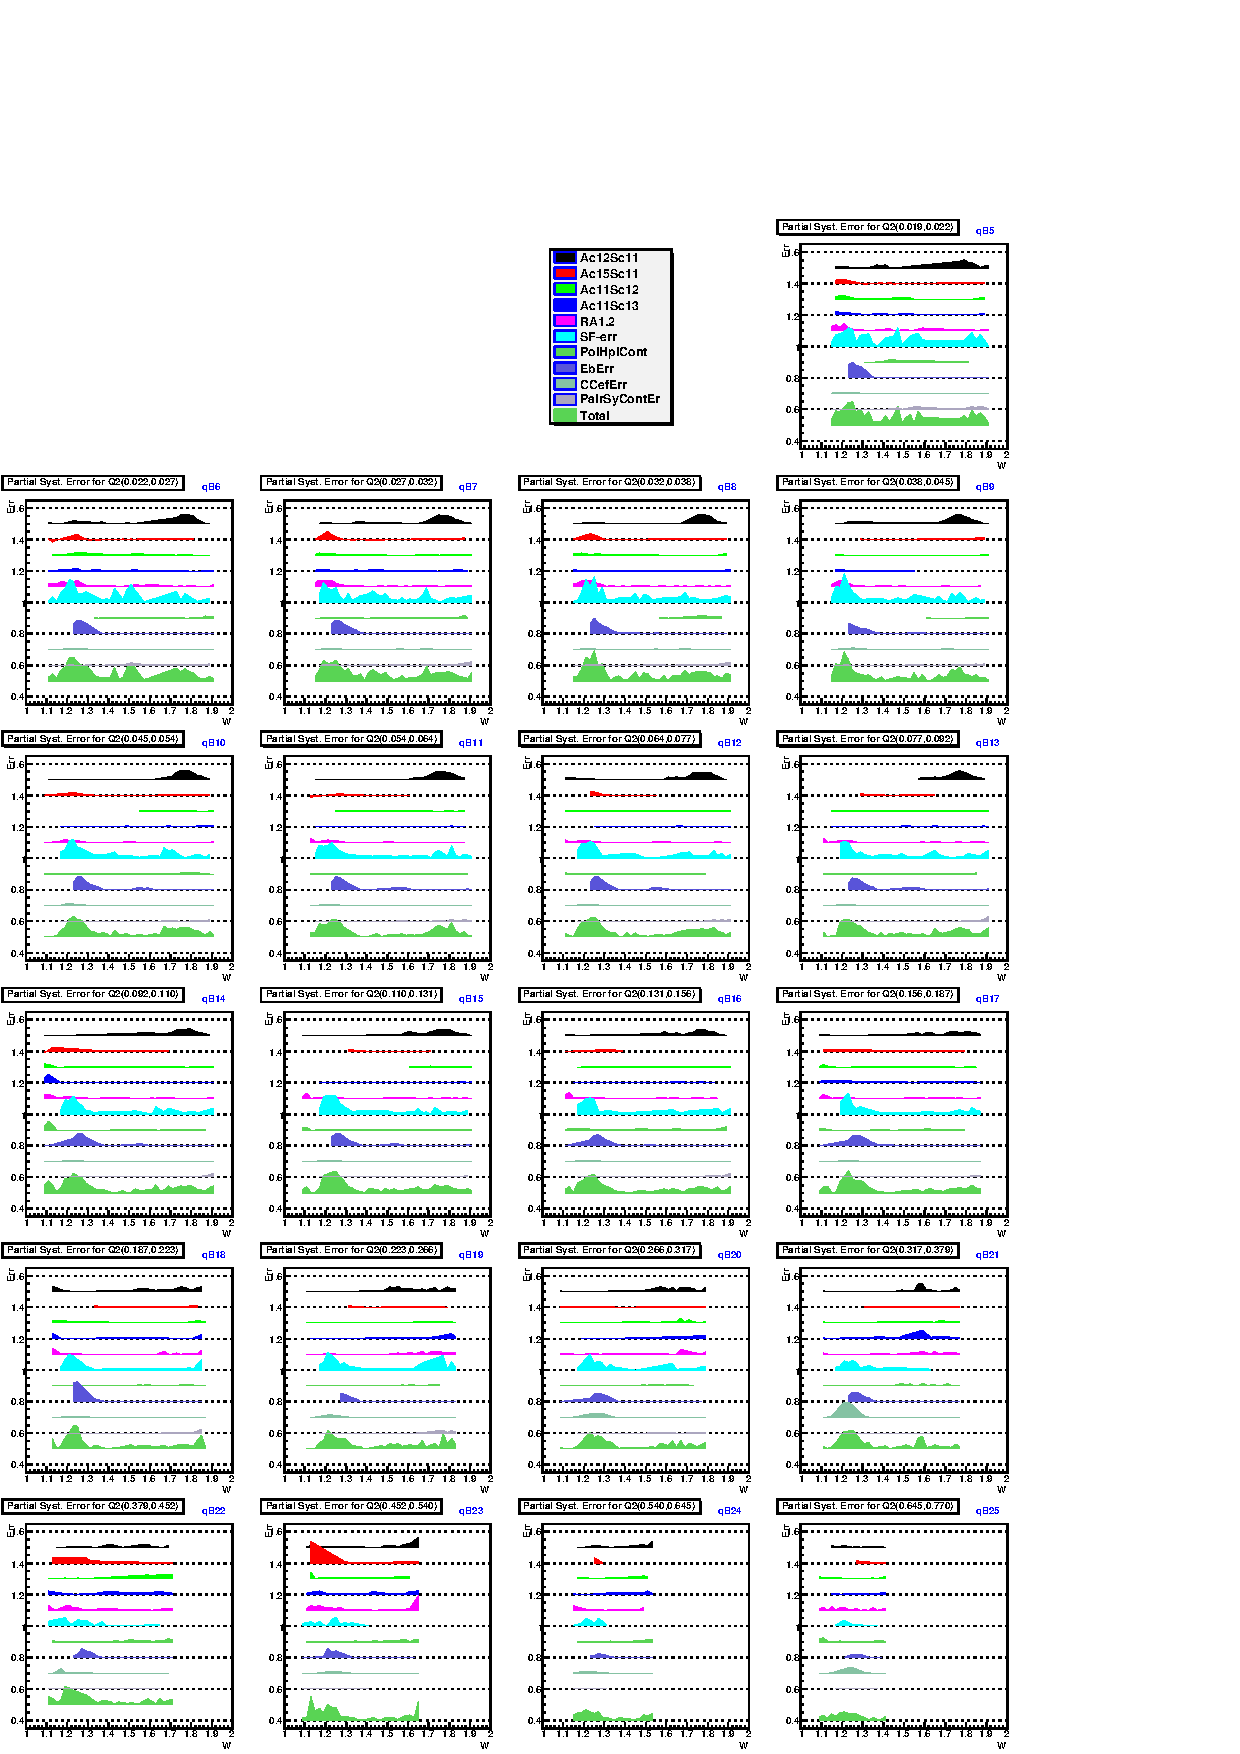
\includegraphics[width=0.95\textwidth]{figuresEG4/FigResults/indvSystErrsA1F1_Eb78Wbins70.png} 
  \leavevmode 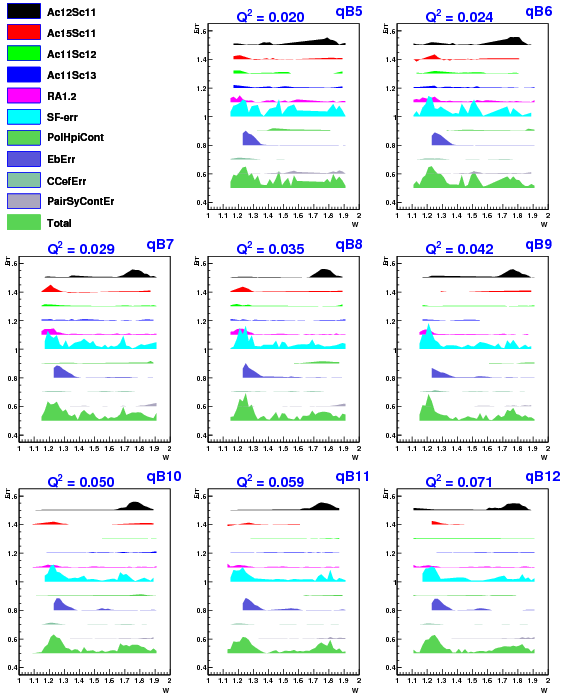
\includegraphics[width=0.95\textwidth]{figuresEG4/FigResults/indvSystErrsA1F1_Eb78Wbins70N.png} 
  \caption[Combined systematic uncertainties in $A_1 F_1$]{Breakdown of systematic uncertainties in $A_1 F_1$ (after combining data from the two energy data sets) in the first few \qsqs bins. See Fig. \ref{sysErEb7q1} for the description of the different systematic uncertainty components.}
  \label{extA1F1SEcomb}  
\end{figure}

\begin{figure}[h] %ht, htpb (p - float, b = bottom, h=? t = top)
\centering
  %\leavevmode 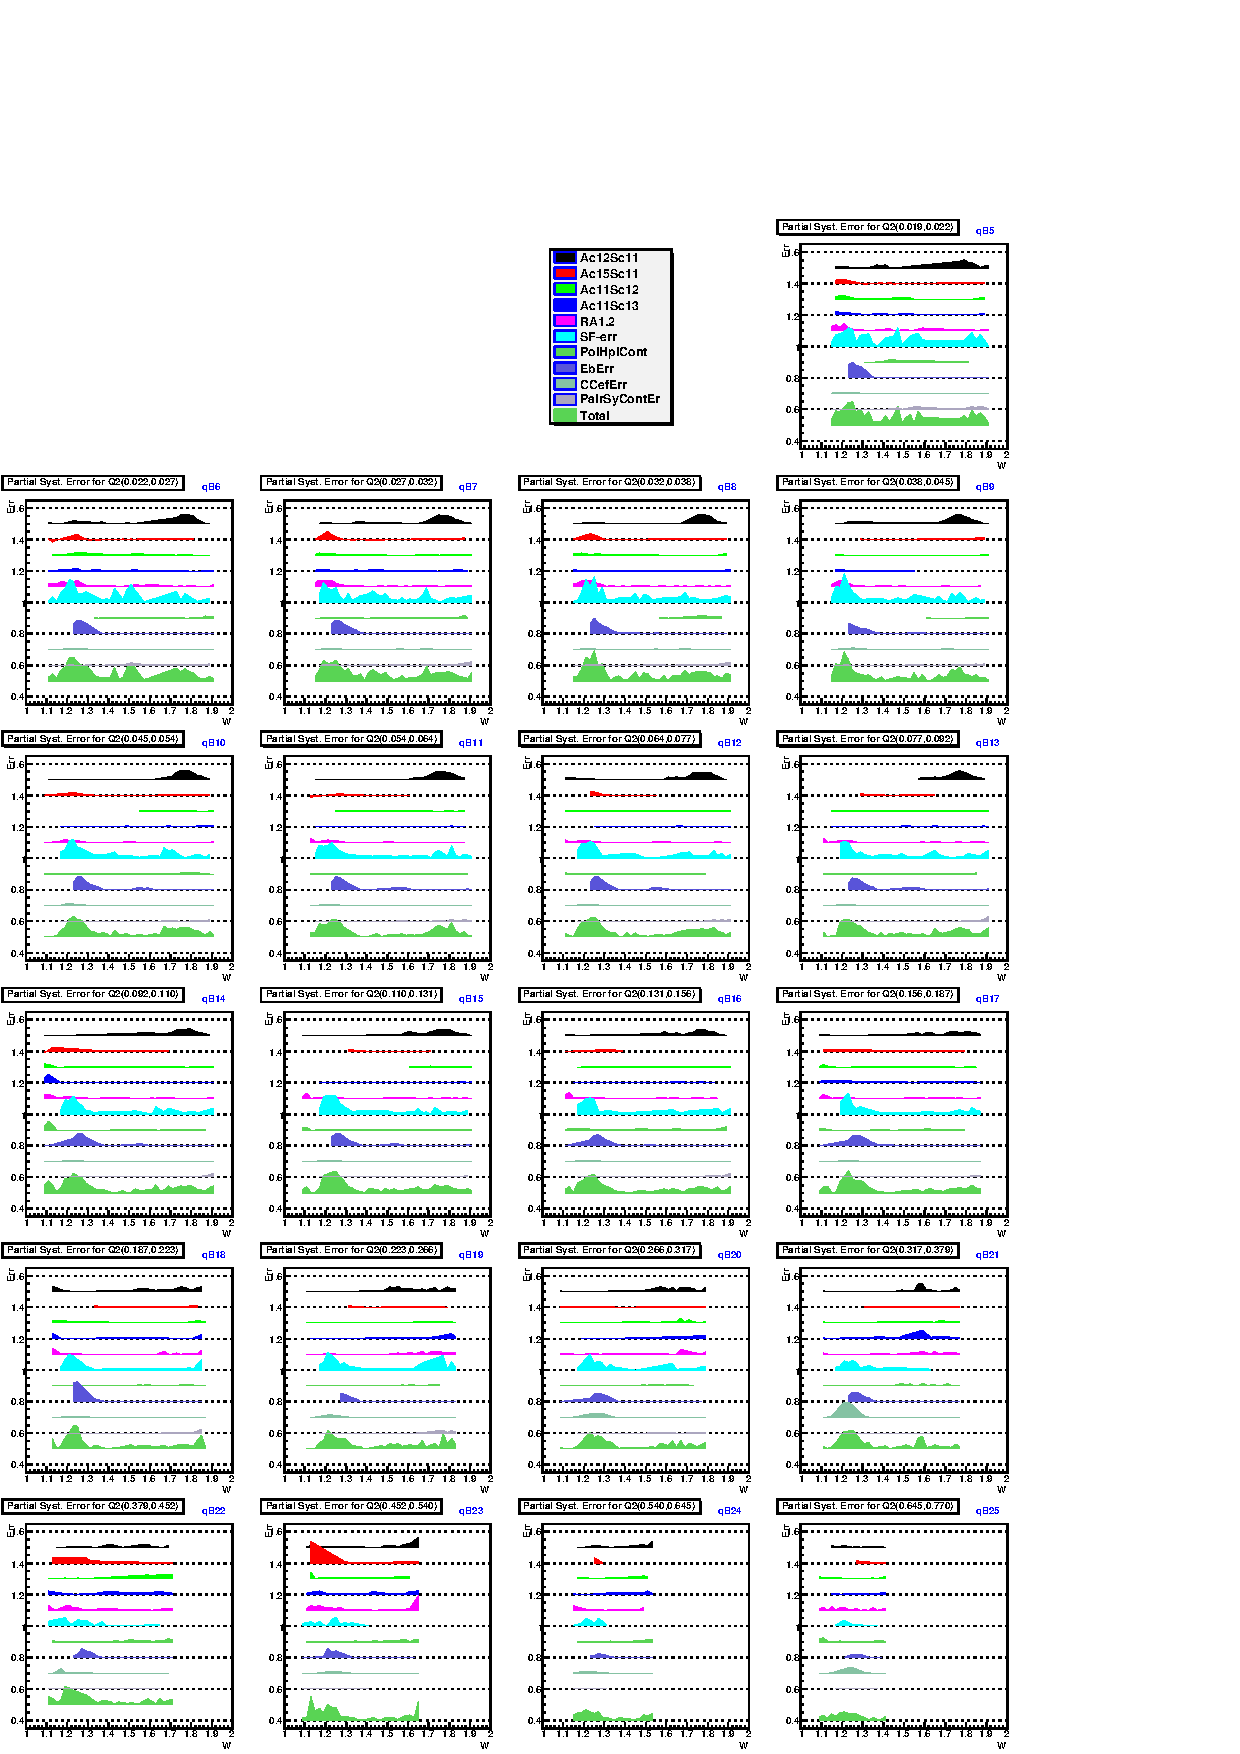
\includegraphics[width=0.95\textwidth]{figuresEG4/FigResults/indvSystErrsA1F1_Eb78Wbins70.png} 
  \leavevmode 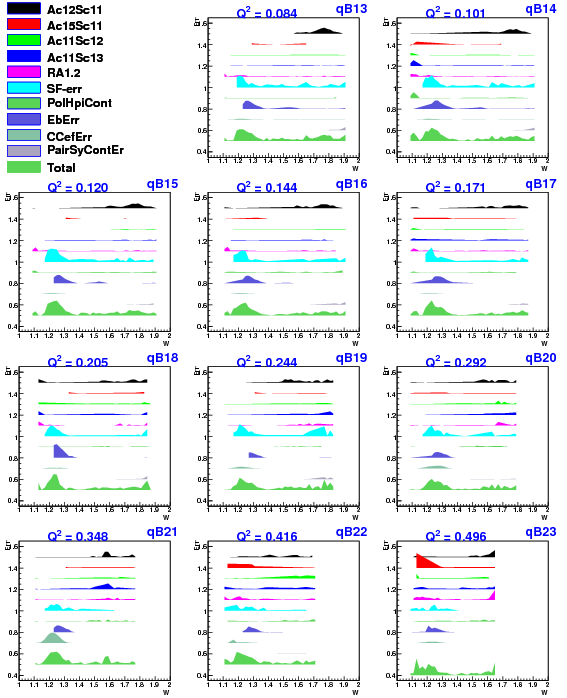
\includegraphics[width=0.95\textwidth]{figuresEG4/FigResults/indvSystErrsA1F1_Eb78Wbins70N2.png} 
  \caption[Combined systematic uncertainties in $A_1 F_1$]{Plots as in Fig. \ref{extA1F1SEcomb}  but in the remaining higher \qsqs bins.}
  \label{extA1F1SEcomb2}  
\end{figure}


\begin{comment} %11/28/13 Dr. Kuhn, why is it here?
%\subsection{Calculation of the integrals and the propagation of the uncertainties}

%The same method translates into the integral, except of course there is no weighting with 1/staterr^2, but instead with Delta-x for each bin. Here, ALL systematic uncertainties are to be treated as correlated, so for all k, you calculate Delta_Gamma1[k, combined] = sum { Delta_g1[k,combined]*Delta-x}.  However, for k = 3,4,5,6 you have to add one more term for the systematic uncertainty for the TOTAL integral (not the data piece): using the SAME variation of the models as you used to calculate the Delta-g1's for these 4 cases, re-calculate the contributions from W = 1.08�1.15 and from W > Wmax by integrating the varied model and subtracting the standard result for those contributions (again, INCLUDING sign). THEN, you can once again add all systematic uncertainties in quadrature
\begin{figure}[h] %ht, htpb (p - float, b = bottom, h=? t = top)
  %\leavevmode 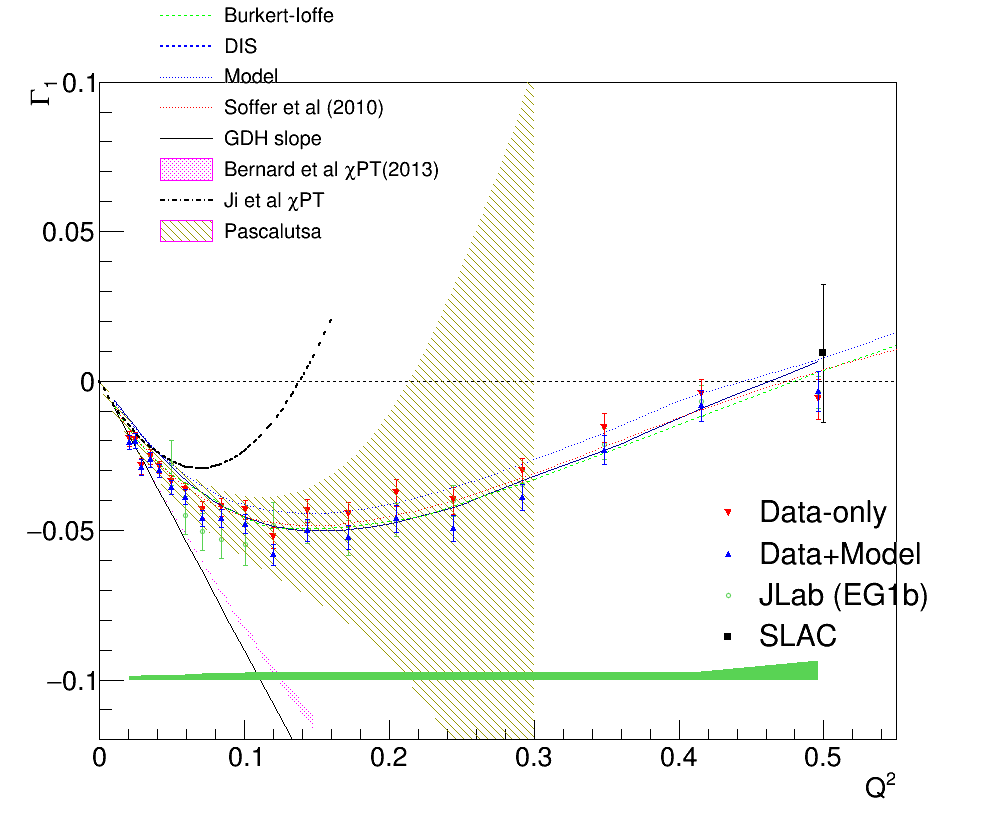
\includegraphics[width=1.0\textwidth]{figuresEG4/FigResults/integralsFromCombinedG1nA1F1_Wbins70Gm1LowQ2.png} 
  \leavevmode 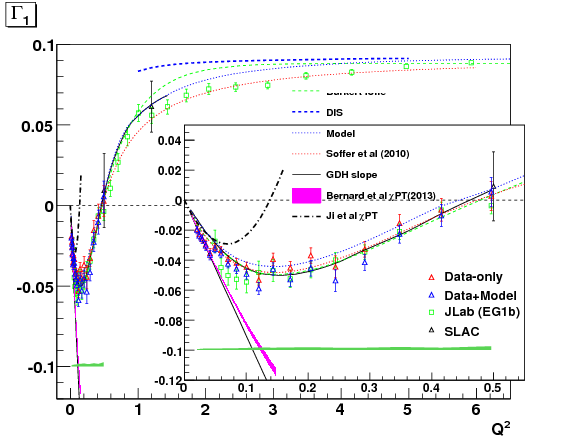
\includegraphics[width=1.0\textwidth]{figuresEG4/FigAnal/integralsFromCombinedG1nA1F1_Wbins70Gm1WdInset.png}
  \caption[Extracted $\Gamma_{1}$]{Extracted $\Gamma_{1}$.}
  \label{extGm1}  
\end{figure}

\end{comment}




%
\clearpage
